\subsection{Network Economics}

A well known concept in neo-classical economy is the \textit{economies of scale}. The larger the company, the lower the price per unit of goods produced. This is known as supply-side economies of scale. Network economics can be briefly defined as \textit{``Stronger gets stronger, weaker gets weaker.''}~\cite{Shapiro1998InformationEconomy} and is interested in the opposite phenomena called \textit{demand-side economies of scale}. The key notion of demand-side economies of scale is the \textit{positive feedback} effect. When two similar technologies are on the market with a similar market share, a slight increase in popularity of one technology can create a perception that this technology is better and will win the entire market. This perception is reflected in the market, where even more consumers choose the slightly more popular technology, raising the market share and strengthening the perception... and so on in a loop, until the technology finally takes over the market. This is known as tipping and can be initiated by an small impulse (e.g. a successful marketing campaign)~\cite{Shapiro1998InformationEconomy}. The market condition over time is illustrated in Firure~\ref{fig:tipping}.

\begin{figure}[ht]
    \centering
    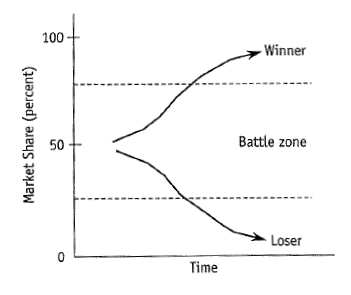
\includegraphics[width=0.6\textwidth]{00images/shapiro}
    \caption{Market during positive feedback. Taken from~\cite{Shapiro1998InformationEconomy}.}
    \label{fig:tipping}
\end{figure}

A typical example is the one of VHS vs. Betamax tapes, where there were two similar (but incompatible) products offered on the market. Minor differences (longer recording time) tipped the market towards VHS, pushing Betamax into the niche zone.

Another factor that can contribute to the positive feedback mechanism are the network externalities. This is particularly visible in communication networks. The more people are connected to a telephony network, the more people can each subscriber call and thus the utility is increased for all participants\footnotemark. However, the networks externalities do not only apply to communication networks. They can just as well be found in use of software (e.g. text editor Microsoft Word), harware (VHS tapes - the ability to borrow tapes from friends) or services (apartment renting -- AirBnB).
% 
\footnotetext{The exact increase in value was expressed as $(n^2)$ in Metcalfe's law. It is however disputed whether this applies in all scenarios and additional models (e.g. $n \times (log\:n)$) were proposed.}
% 

\paragraph{Network effect in cloud-based machine learning services} In current market practice, cloud based solution by the major cloud providers usually offer variety of services, apart from \acrshort{ml}. The Azure cloud solution by Microsoft\footnotemark~for example offers over 200 different tools and products, all hosted on the cloud. The competing solutions are similar. If a customer were to use a cloud based \acrshort{ml} solution by either of the big market players, they could easily integrate their model with the other tools in the portfolio of the same provider.
% 
\footnotetext{\url{https://azure.microsoft.com/en-us/}, accessed 10-12-2018}
% 
Moreover, the main \acrshort{ml} services by different providers are not compatible with each other, further increasing the switching cost and supporting the tipping scenario\footnotemark.
% 
\footnotetext{We have to note that some parts of the cloud-based \acrshort{ml} services build on top of industry standards which are shared and supported by all the major players. Further analysis would be necessary to exactly determine the degree to which a ready solution on one platform can be fully migrated to another platform.}